\ifx\PREAMBLE\undefined
\documentclass{article}
\usepackage[format = hang, font = bf]{caption}
\usepackage{graphicx}
\usepackage{array}
\usepackage{amsmath}
\usepackage{mathtools}
\usepackage{boxedminipage}
\usepackage{listings}
\usepackage{makecell}%diagonal line in table
\usepackage{float}%allowing forceful figure[H]
\usepackage{xcolor}
\usepackage{amsfonts}%allowing \mathbb{R}
\usepackage{alltt}
\usepackage{url}
\def\UrlBreaks{\do\A\do\B\do\C\do\D\do\E\do\F\do\G\do\H\do\I\do\J\do\K\do\L\do\M\do\N\do\O\do\P\do\Q\do\R\do\S\do\T\do\U\do\V\do\W\do\X\do\Y\do\Z\do\[\do\\\do\]\do\^\do\_\do\`\do\a\do\b\do\c\do\d\do\e\do\f\do\g\do\h\do\i\do\j\do\k\do\l\do\m\do\n\do\o\do\p\do\q\do\r\do\s\do\t\do\u\do\v\do\w\do\x\do\y\do\z\do\0\do\1\do\2\do\3\do\4\do\5\do\6\do\7\do\8\do\9\do\.\do\@\do\\\do\/\do\!\do\_\do\|\do\;\do\>\do\]\do\)\do\,\do\?\do\'\do+\do\=\do\#\do\-}
\usepackage[breaklinks = true]{hyperref}
\lstset{language = matlab, breaklines = true, tabsize = 2, numbers = left, extendedchars = false, basicstyle = {\ttfamily \footnotesize}, keywordstyle=\color{blue!70}, commentstyle=\color{red!70}, frame=shadowbox, rulesepcolor=\color{red!20!green!20!blue!20}, numberstyle={\color[RGB]{0,192,192}}}

\begin{document}
\fi
\section{Support vector machine (SVM)}
\subsection{Cost function}
Recall the cost function of logistic regression:
\begin{equation}
\begin{split}
J(\theta) = &\frac{1}{m}\sum\limits_{i=1}^{m}\left(-y^{(i)}\log\frac{1}{1+e^{-\theta^{\mathsf T}x^{(i)}}} - (1-y^{(i)})\log\left(1-\frac{1}{1+e^{-\theta^{\mathsf T}x^{(i)}}}\right)\right) \\
&+ \frac{\lambda}{2m}\sum\limits_{j=1}^{n}\theta_j^{2}
\end{split}\end{equation}
For a training example $(x,y)$ with $y=1$, we expect $\theta^{\mathsf T}x\gg 0$ in order to minimize the cost function. Similarly, we expect $\theta^{\mathsf T}x\ll 0$ for an example with $y=0$. The graph of $f_1(z) = -\log\frac{1}{1+e^{-z}}$ is provided with the blue line in Figure \ref{cost1}, while the graph of $f_0(z) = -\log\left(1-\frac{1}{1+e^{-z}}\right)$ is provided with the blue line in Figure \ref{cost0}.
\begin{figure}[H]
\centering
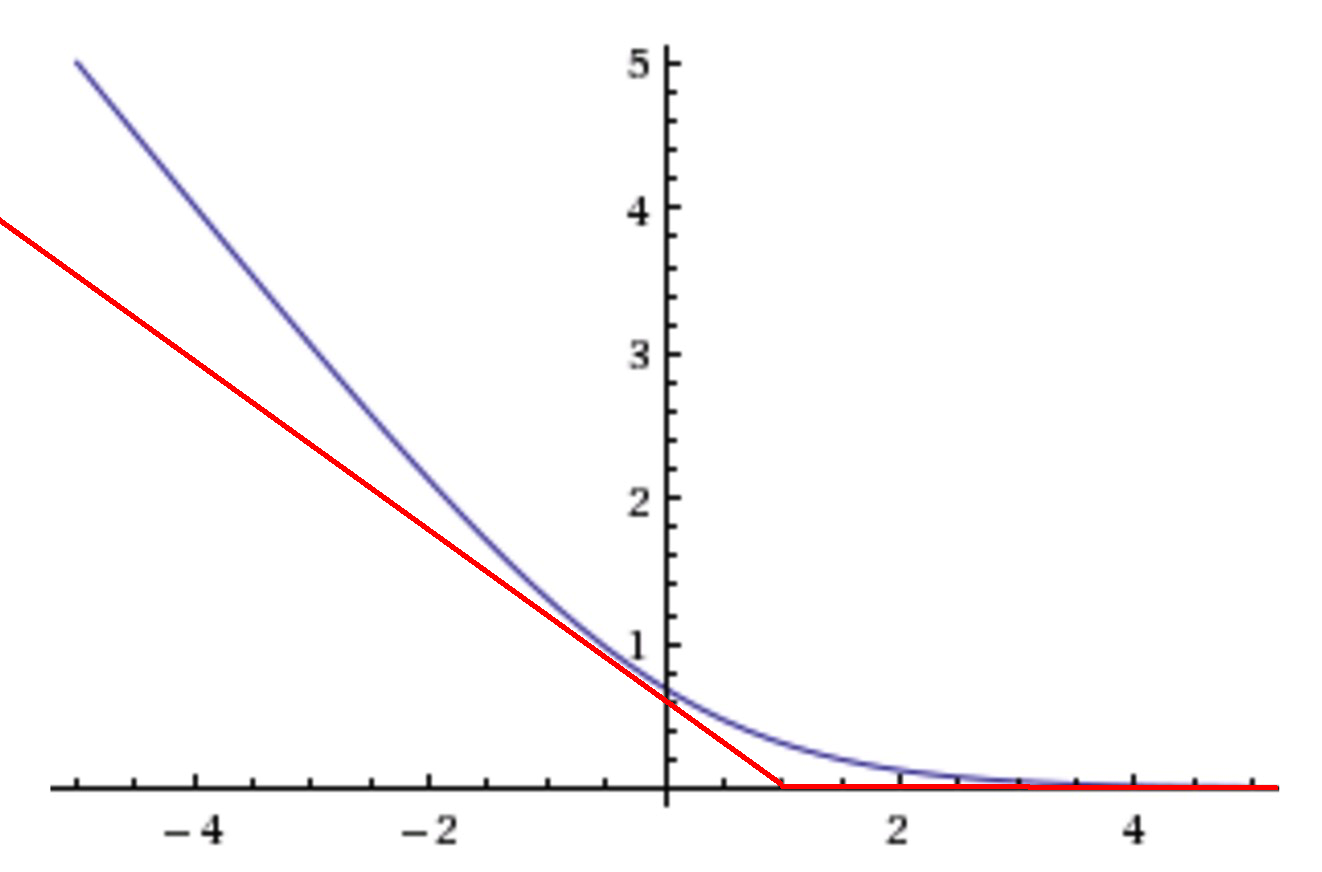
\includegraphics[width = 0.6\textwidth]{cost1.jpg}
\caption{Image of cost1(z)}\label{cost1}
\end{figure}
\begin{figure}[H]
\centering
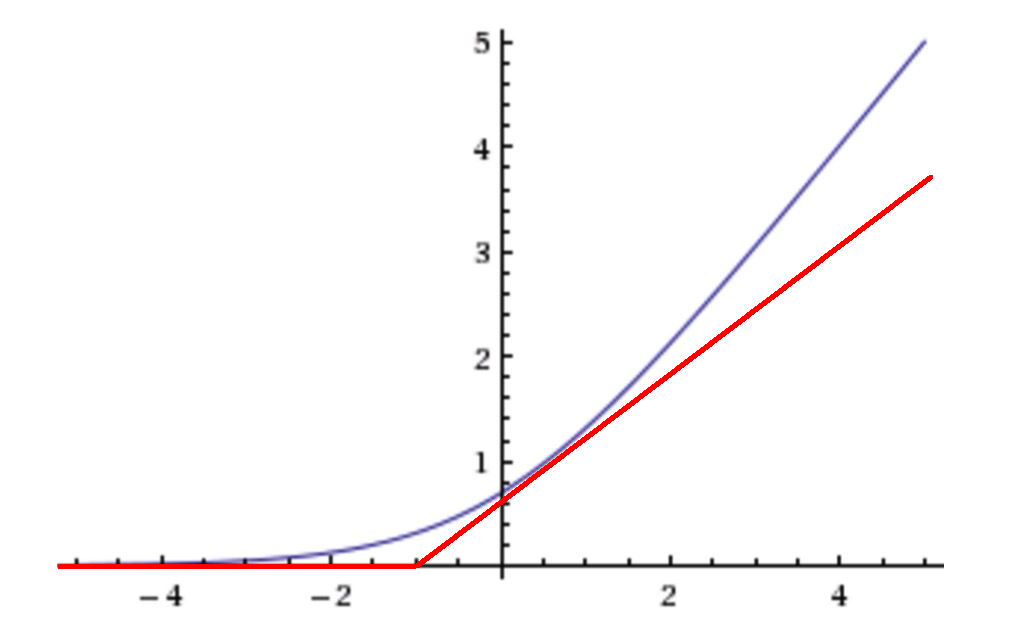
\includegraphics[width = 0.6\textwidth]{cost0.jpg}
\caption{Image of cost0(z)}\label{cost0}
\end{figure}
In SVM, we will use new functions $cost1(z), cost0(z)$ as depicted by the red lines in Figure \ref{cost1} and Figure \ref{cost0} to substitute $f_1(z)$ and $f_0(z)$. The new cost function is 
\begin{equation}
J(\theta) = C\sum\limits_{i=1}^{m}\left(y^{(i)}cost1(\theta^{\mathsf T}x^{(i)}) + (1-y^{(i)})cost0(\theta^{\mathsf T}x^{(i)})\right) + \frac{1}{2}\sum\limits_{j=1}^{n}\theta_j^{2}
\end{equation}
Note that for the reason of convention, $m$ is dropped and rather than writing the function as $A + \lambda B$, we are now writing it as $CA + B$. $C$ has the same effect as the original $\frac{1}{\lambda}$ when it comes to its effect on regularization.

Unlike logistic regression, in which $h_{\theta}(x)$ is interpreted as the probablity of $y=1$, SVM has the following hypothesis:
\begin{equation}
h_{\theta}(x) = \left\{
\begin{aligned}
1,& \text{ if } \theta^{\mathsf T}x \ge 0\\
0,& \text{ otherwise}
\end{aligned}
\right.
\end{equation}
\subsection{Large margin classification}
It is easy to tell from the graphs of $cost1$ and $cost0$ that for a training example with $y=1$, in order to minimize the cost function, we expect $\theta^{\mathsf T}x \ge 1$(not just $\ge 0$). If $y=0$, we expect $\theta^{\mathsf T}x \le -1$(not just $<0$). This builds an extra ``safety margin factor'' for the SVM. Geometrically, in a linearly separable case, it is ralated to choosing the decision boundary that maximizes its distance from the examples, i.e. conducts the ``large margin classification''. Figure \ref{largemargin} demonstrates a simple case. Here, large margin classification results in the green line as the decision boundary, rather than the black one or the orange one. 
\begin{figure}[H]
\centering
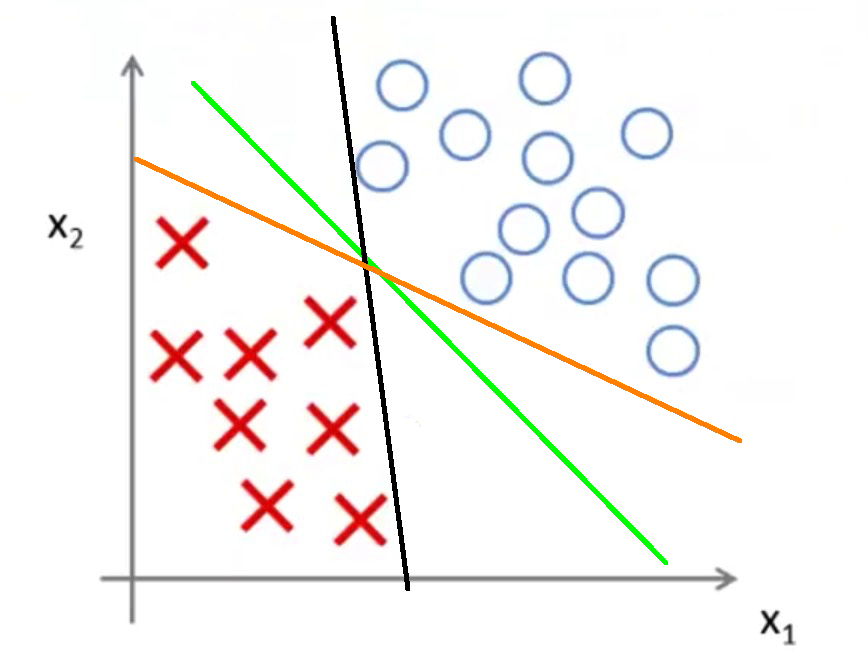
\includegraphics[width = 0.6\textwidth]{largemargin.jpg}
\caption{Intuition of large margin classification}\label{largemargin}
\end{figure}
When there exist outliners, the regularization factor $C$ ensures that the algorithm does not overfit the examples. Obviously $C$ cannot be too large.
\begin{figure}[H]
\centering
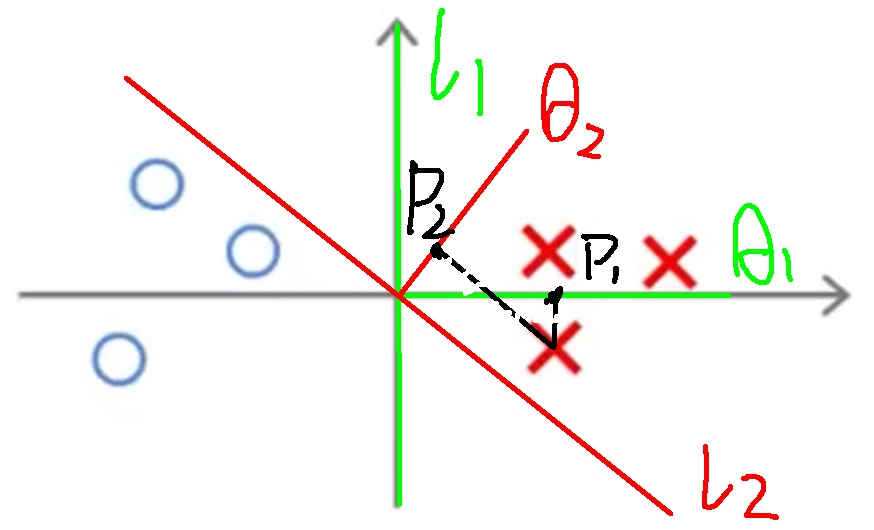
\includegraphics[width = 0.6\textwidth]{largemarginmath.jpg}
\caption{Mathematical background of large margin classification}\label{largemarginmath}
\end{figure}
The mathematical background of large margin classification can be illustrated by Figure \ref{largemarginmath}. In this simple 2-d case, our target becomes
\begin{equation}
\begin{split}
&\min\limits_{\theta}\frac{1}{2}\sum\limits_{j=1}^{n}\theta_j^2=\min\limits_{\theta}\frac{1}{2}\lVert\theta\rVert^2\\
&\text{ s.t. }\left\{
\begin{aligned}
\theta^{\mathsf T}x^{(i)} \ge& 1, \text{ if }y^{(i)} = 1\\
\theta^{\mathsf T}x^{(i)} \le& -1, \text{ if }y^{(i)} = 0
\end{aligned}\right.
\end{split}
\end{equation}
Note that 
$$\theta^{\mathsf T}x= \lVert\theta\rVert\lVert x\rVert\cos\langle\theta,x\rangle = p\cdot \lVert\theta\rVert$$
in which $p$ is the projection of $x$ along the direction of $\theta$. In order to minimize $\lVert\theta\rVert$, $p$ should be as large as possible for all samples. From Figure \ref{largemarginmath}, obviously $l_1$ is a better decision boundary because $p_1>p_2$.
\subsection{Kernals}
In order to adapt SVMs to develop complex non-linear classifiers, we have to use {\bf kernals}.

One way to develop non-linear classifiers is to use high degree polynomial features. We will end up with a classifier that predicts $y=1$ if 
\begin{equation}\label{polyfeatures}
\theta_0 + \theta_1x_1 + \theta_2x_2 + \theta_3x_1^2 + \theta_4x_2^2 + \theta_5x_1x_2 + \dots > 0
\end{equation}
\eqref{polyfeatures} can also be written as 
$$\theta^{\mathsf T}f > 0$$
in which
\begin{equation*}
\begin{bmatrix}
f_1\\
f_2\\
f_3\\
f_4\\
f_5\\
\dots
\end{bmatrix}=
\begin{bmatrix}
x_1\\
x_2\\
x_1^2\\
x_2^2\\
x_1x_2\\
\dots
\end{bmatrix}
\end{equation*}
In complex cases, there could be a lot of polynomial features, causing significant computational difficulty. Our target is to find a better choice of features $f_1, f_2, f_3\dots$

Kernal introduces the idea to compute features of an example $x$ according to its proximity to a series of landmarks $l^{(i)}$, e.g.
\begin{equation}
f_i = \text{similarity}\left(x,l^{(i)}\right) = \exp\left(-\frac{\lVert x-l^{(i)}\rVert^2}{2\sigma^2}\right)
\end{equation}
Here we are using {\bf Gaussian Kernal}. When $x$ is close to $l^{(i)}$, this kernal returns approximately 1, while when $x$ is far from $l^{(i)}$, it returns approximately 0.

With featurs $f_i$ defined as such, we now have SVMs that can conduct non-linear classification. The SVM predicts $y=1$ when $\theta^{\mathsf T}f \ge 0$, and $y=0$ otherwise.

As for the choice of landmarks $l^{(i)}$, in practice, we use all examples in the training set as landmarks. Thus we will end up with $m$ features. $\theta$ can be trained with
\begin{equation}
\min\limits_{\theta}C\sum\limits_{i=1}^{m}\left(y^{(i)}cost1(\theta^{\mathsf T}f^{(i)}) + (1- y^{(i)})cost0(\theta^{\mathsf T}f^{(i)})\right) + \frac{1}{2}\sum\limits_{i=1}^{m}\theta_i^2
\end{equation}
Since we have exactly $m$ features, now we have $n=m$. 

As mentioned above, $C$ controls the regularization in the same way as $\frac{1}{\lambda}$ before. Thus with large $C$, the SVM tends to have high variance and low bias, whereas with small $C$, it tends to have high bias and low variance. The $\sigma$ in the definition of Gaussion kernal also affects the bias and variance of the SVM. With large $\sigma$, features vary more smoothly, and the SVM tends to have high bias and low variance, while with small $\sigma$, features vary more rapidly, and it tends to have high variance and low bias.

When using Gaussian kernal, it is important to do feature scaling. Otherwise $\lVert x-l\rVert^2$ will be dominated by the component with largest magnitude.
\subsection{Logistic regression v.s. SVM}
Some guidelines about the choice between logistic regression and SVM:
\begin{itemize}
\item When $n$ is large and $m$ is small: use logistic regression or SVM without a kernal (linear kernal).
\item When $n$ is small and $m$ is large: add/create more features and then use logistic regression or SVM without a kernal.
\item When $n$ is small and $m$ is intermediate: use SVM with Gaussian kernal. 
\end{itemize}

\ifx\PREAMBLE\undefined
\end{document}
\fi